\documentclass[11pt]{standalone}
\usepackage[usenames]{color} %used for font color
\usepackage{amssymb} %maths
\usepackage{amsmath} %maths
\usepackage[no-math]{fontspec}
\setmainfont{Lato}
\usepackage{unicode-math}
\usepackage{tikz}
\usetikzlibrary{positioning,shapes.geometric}
% Farben definieren
\definecolor{background}{HTML}{F3F4F4}
\definecolor{inputneuron}{HTML}{CCDEE9}
\definecolor{outputneuron}{HTML}{005A94}
\begin{document}
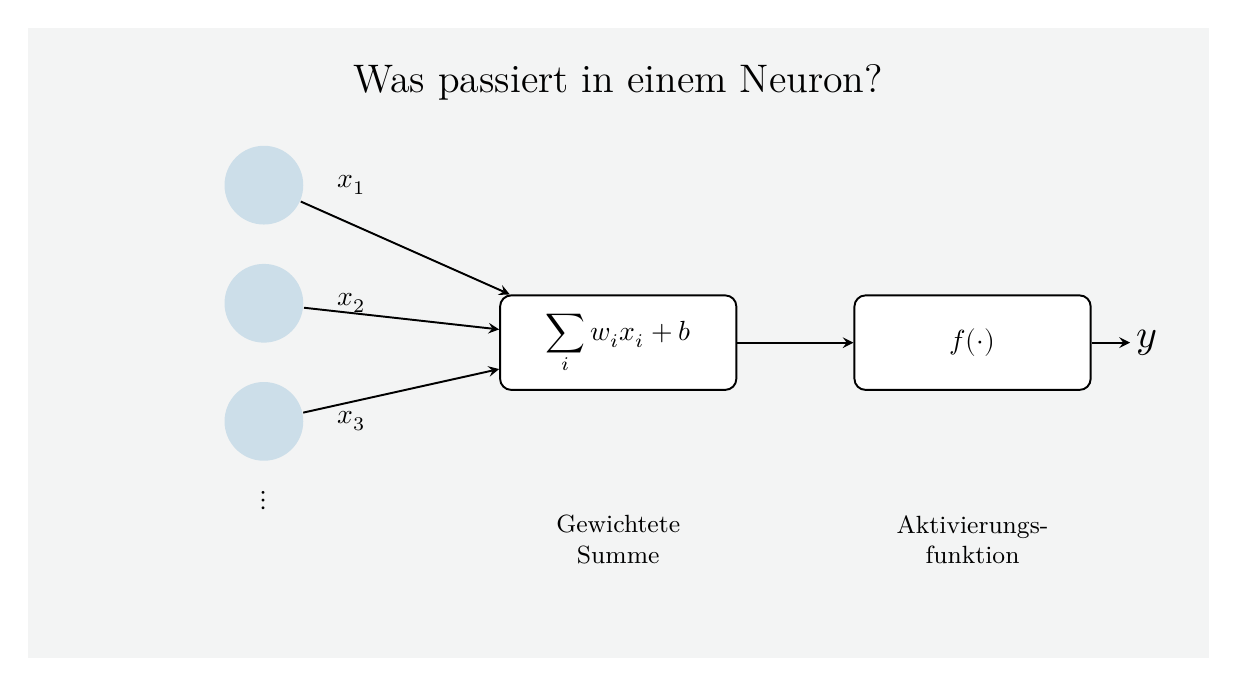
\begin{tikzpicture}[
    % Stile definieren
    neuron/.style={circle, minimum size=1cm, draw=black, line width=0.7pt},
    input neuron/.style={neuron, fill=inputneuron, draw=none},
    process/.style={rectangle, rounded corners, minimum width=3cm, minimum height=1.2cm, 
                    draw=black, line width=0.7pt, fill=white},
    connection/.style={draw=black, line width=0.7pt, -stealth}
]
% Hintergrund
\fill[background] (-3,-4) rectangle (12,4);

% Titel
\node[font=\Large] at (4.5,3.3) {Was passiert in einem Neuron?};

% Eingänge links
\node[input neuron] (x1) at (0,2) {};
\node[font=\normalsize, right=0.3cm of x1] {$x_1$};
\node[input neuron] (x2) at (0,0.5) {};
\node[font=\normalsize, right=0.3cm of x2] {$x_2$};
\node[input neuron] (x3) at (0,-1) {};
\node[font=\normalsize, right=0.3cm of x3] {$x_3$};
\node[font=\normalsize] at (0,-2) {$\vdots$};

% Gewichtete Summe
\node[process] (sum) at (4.5,0) {$\displaystyle\sum_{i} w_i x_i + b$};

% Aktivierungsfunktion
\node[process] (activation) at (9,0) {$f(\cdot)$};

% Ausgabe
\node[font=\Large] at (11.2,0) {$y$};

% Verbindungen
\draw[connection] (x1) -- (sum);
\draw[connection] (x2) -- (sum);
\draw[connection] (x3) -- (sum);

\draw[connection] (sum) -- (activation);
\draw[connection] (activation) -- (11,0);

% Beschriftungen unter den Boxen
\node[font=\small, align=center] at (4.5,-2.5) {Gewichtete\\Summe};
\node[font=\small, align=center] at (9,-2.5) {Aktivierungs-\\funktion};

\end{tikzpicture}
\end{document}
